% Options for packages loaded elsewhere
\PassOptionsToPackage{unicode}{hyperref}
\PassOptionsToPackage{hyphens}{url}
\documentclass[
  ignorenonframetext,
]{beamer}
\newif\ifbibliography
\usepackage{pgfpages}
\setbeamertemplate{caption}[numbered]
\setbeamertemplate{caption label separator}{: }
\setbeamercolor{caption name}{fg=normal text.fg}
\beamertemplatenavigationsymbolsempty
% remove section numbering
\setbeamertemplate{part page}{
  \centering
  \begin{beamercolorbox}[sep=16pt,center]{part title}
    \usebeamerfont{part title}\insertpart\par
  \end{beamercolorbox}
}
\setbeamertemplate{section page}{
  \centering
  \begin{beamercolorbox}[sep=12pt,center]{section title}
    \usebeamerfont{section title}\insertsection\par
  \end{beamercolorbox}
}
\setbeamertemplate{subsection page}{
  \centering
  \begin{beamercolorbox}[sep=8pt,center]{subsection title}
    \usebeamerfont{subsection title}\insertsubsection\par
  \end{beamercolorbox}
}
% Prevent slide breaks in the middle of a paragraph
\widowpenalties 1 10000
\raggedbottom
\AtBeginPart{
  \frame{\partpage}
}
\AtBeginSection{
  \ifbibliography
  \else
    \frame{\sectionpage}
  \fi
}
\AtBeginSubsection{
  \frame{\subsectionpage}
}
\usepackage{iftex}
\ifPDFTeX
  \usepackage[T1]{fontenc}
  \usepackage[utf8]{inputenc}
  \usepackage{textcomp} % provide euro and other symbols
\else % if luatex or xetex
  \usepackage{unicode-math} % this also loads fontspec
  \defaultfontfeatures{Scale=MatchLowercase}
  \defaultfontfeatures[\rmfamily]{Ligatures=TeX,Scale=1}
\fi
\usepackage{lmodern}
\ifPDFTeX\else
  % xetex/luatex font selection
\fi
% Use upquote if available, for straight quotes in verbatim environments
\IfFileExists{upquote.sty}{\usepackage{upquote}}{}
\IfFileExists{microtype.sty}{% use microtype if available
  \usepackage[]{microtype}
  \UseMicrotypeSet[protrusion]{basicmath} % disable protrusion for tt fonts
}{}
\makeatletter
\@ifundefined{KOMAClassName}{% if non-KOMA class
  \IfFileExists{parskip.sty}{%
    \usepackage{parskip}
  }{% else
    \setlength{\parindent}{0pt}
    \setlength{\parskip}{6pt plus 2pt minus 1pt}}
}{% if KOMA class
  \KOMAoptions{parskip=half}}
\makeatother
\usepackage{longtable,booktabs,array}
\newcounter{none} % for unnumbered tables
\usepackage{calc} % for calculating minipage widths
\usepackage{caption}
% Make caption package work with longtable
\makeatletter
\def\fnum@table{\tablename~\thetable}
\makeatother
\usepackage{graphicx}
\makeatletter
\newsavebox\pandoc@box
\newcommand*\pandocbounded[1]{% scales image to fit in text height/width
  \sbox\pandoc@box{#1}%
  \Gscale@div\@tempa{\textheight}{\dimexpr\ht\pandoc@box+\dp\pandoc@box\relax}%
  \Gscale@div\@tempb{\linewidth}{\wd\pandoc@box}%
  \ifdim\@tempb\p@<\@tempa\p@\let\@tempa\@tempb\fi% select the smaller of both
  \ifdim\@tempa\p@<\p@\scalebox{\@tempa}{\usebox\pandoc@box}%
  \else\usebox{\pandoc@box}%
  \fi%
}
% Set default figure placement to htbp
\def\fps@figure{htbp}
\makeatother
\setlength{\emergencystretch}{3em} % prevent overfull lines
\providecommand{\tightlist}{%
  \setlength{\itemsep}{0pt}\setlength{\parskip}{0pt}}
% Slide layout defaults for warning-clean scientific decks.
\usepackage{etoolbox}
\IfFileExists{xurl.sty}{\usepackage{xurl}}{}
\IfFileExists{seqsplit.sty}{\usepackage{seqsplit}}{\newcommand{\seqsplit}[1]{#1}}
\protected\def\breakseq#1{\seqsplit{#1}}
\protected\def\breaktt#1{\begingroup\ttfamily\seqsplit{#1}\endgroup}
\setlength{\emergencystretch}{6em}
\tolerance=5000
\hbadness=10000
\hfuzz=1pt
\setlength{\tabcolsep}{2pt}
\AtBeginEnvironment{longtable}{\tiny\renewcommand{\arraystretch}{0.86}\setlength{\tabcolsep}{1pt}}
\AtBeginEnvironment{tabular}{\tiny\renewcommand{\arraystretch}{0.86}\setlength{\tabcolsep}{1pt}}

% Natbib and cross-reference fallbacks — slides don't load natbib
% or cleveref, but combined-PDF manuscript prose may emit these
% commands. The fallback renders citations as a bracketed key list
% and cross-references as detokenized labels so slides don't fail on
% undefined control sequences or raw underscores. \providecommand is
% a no-op if packages load later.
\providecommand{\citep}[1]{[#1]}
\providecommand{\citet}[1]{#1}
\providecommand{\citealp}[1]{#1}
\providecommand{\citeauthor}[1]{#1}
\providecommand{\citeyear}[1]{#1}
\providecommand{\cref}[1]{\texttt{\detokenize{#1}}}
\providecommand{\Cref}[1]{\texttt{\detokenize{#1}}}

\newtheorem{proposition}{Proposition}
\newtheorem{hypothesis}{Hypothesis}
\usepackage{bookmark}
\IfFileExists{xurl.sty}{\usepackage{xurl}}{} % add URL line breaks if available
\urlstyle{same}
% fallback for those not using the hyperref driver hyperxmp:
\makeatletter
\@ifundefined{xmpquote}{\newcommand{\xmpquote}[1]{#1}}{}
\makeatother
\hypersetup{
  hidelinks,
  pdfcreator={LaTeX via pandoc}}

\author{\texorpdfstring{}{}}
\date{}

\begin{document}

\section{Introduction}\label{introduction}

\begin{frame}[fragile,allowframebreaks]{Motivation}
\protect\phantomsection\label{motivation}
Modern research software repositories increasingly adopt monorepo
designs in which multiple projects share a common set of curated
resources. A monorepo consolidates source code, documentation, datasets,
and governance artefacts under one version-controlled root, enabling
atomic cross-project changes and a single source of truth for shared
data \breakseq{[@Fowler2002patterns]}. The practical benefit is significant: a
bibliography updated once in
\breaktt{fonds/templates/template\_bibliography/} is immediately
available to every project that discovers it at runtime, without any
per-project copy.

Three categories of shared resource appear consistently across research
template repositories:

\begin{enumerate}
\tightlist
\item
  \textbf{Data pools (fonds)}: curated reference sets ---
  bibliographies, contact registries, dataset catalogues --- that
  projects query but must never mutate.
\item
  \textbf{Governance rules}: machine-readable constraint schemas and
  human-readable style guidelines that projects load to validate their
  own outputs.
\item
  \textbf{Executable tools}: script-based entry points that projects
  invoke to run computations, validate artefacts, or call external
  agents.
\end{enumerate}

Without a canonical integration pattern for consuming these resources,
projects face a dilemma: they can hard-code discovery paths (creating
fragile, repo-root-sensitive logic) or skip resource consumption
entirely (forfeiting the monorepo's collaborative benefits). Neither
outcome is acceptable in a public, forkable template repository intended
to demonstrate best practices \breakseq{[@Wilson2014best]}.
\end{frame}

\begin{frame}[fragile,allowframebreaks]{Contribution}
\protect\phantomsection\label{contribution}
This paper introduces \breaktt{template\_pools\_rules\_tools}, a
\textbf{meta-project exemplar} that resolves this dilemma with a
four-module architecture (@fig:architecture). Each module handles one
resource category plus a fourth orchestration module:

{\def\LTcaptype{none} % do not increment counter
\begin{longtable}[]{@{}
  >{\raggedright\arraybackslash}p{(\linewidth - 4\tabcolsep) * \real{0.3333}}
  >{\raggedright\arraybackslash}p{(\linewidth - 4\tabcolsep) * \real{0.3333}}
  >{\raggedright\arraybackslash}p{(\linewidth - 4\tabcolsep) * \real{0.3333}}@{}}
\toprule\noalign{}
\begin{minipage}[b]{\linewidth}\raggedright
Module
\end{minipage} & \begin{minipage}[b]{\linewidth}\raggedright
Resource category
\end{minipage} & \begin{minipage}[b]{\linewidth}\raggedright
Key function
\end{minipage} \\
\midrule\noalign{}
\endhead
\breaktt{src/fonds\_reader.py} & Data pools &
\breaktt{read\_all\_fonds()} \\
\breaktt{src/rules\_applier.py} & Governance rules &
\breaktt{validate\_against\_rules()} \\
\breaktt{src/tools\_invoker.py} & Executable tools &
\breaktt{discover\_tools()} \\
\breaktt{src/integration.py} & All three &
\breaktt{run\_integration\_demo()} \\
\bottomrule\noalign{}
\end{longtable}
}

\begin{figure}
\centering
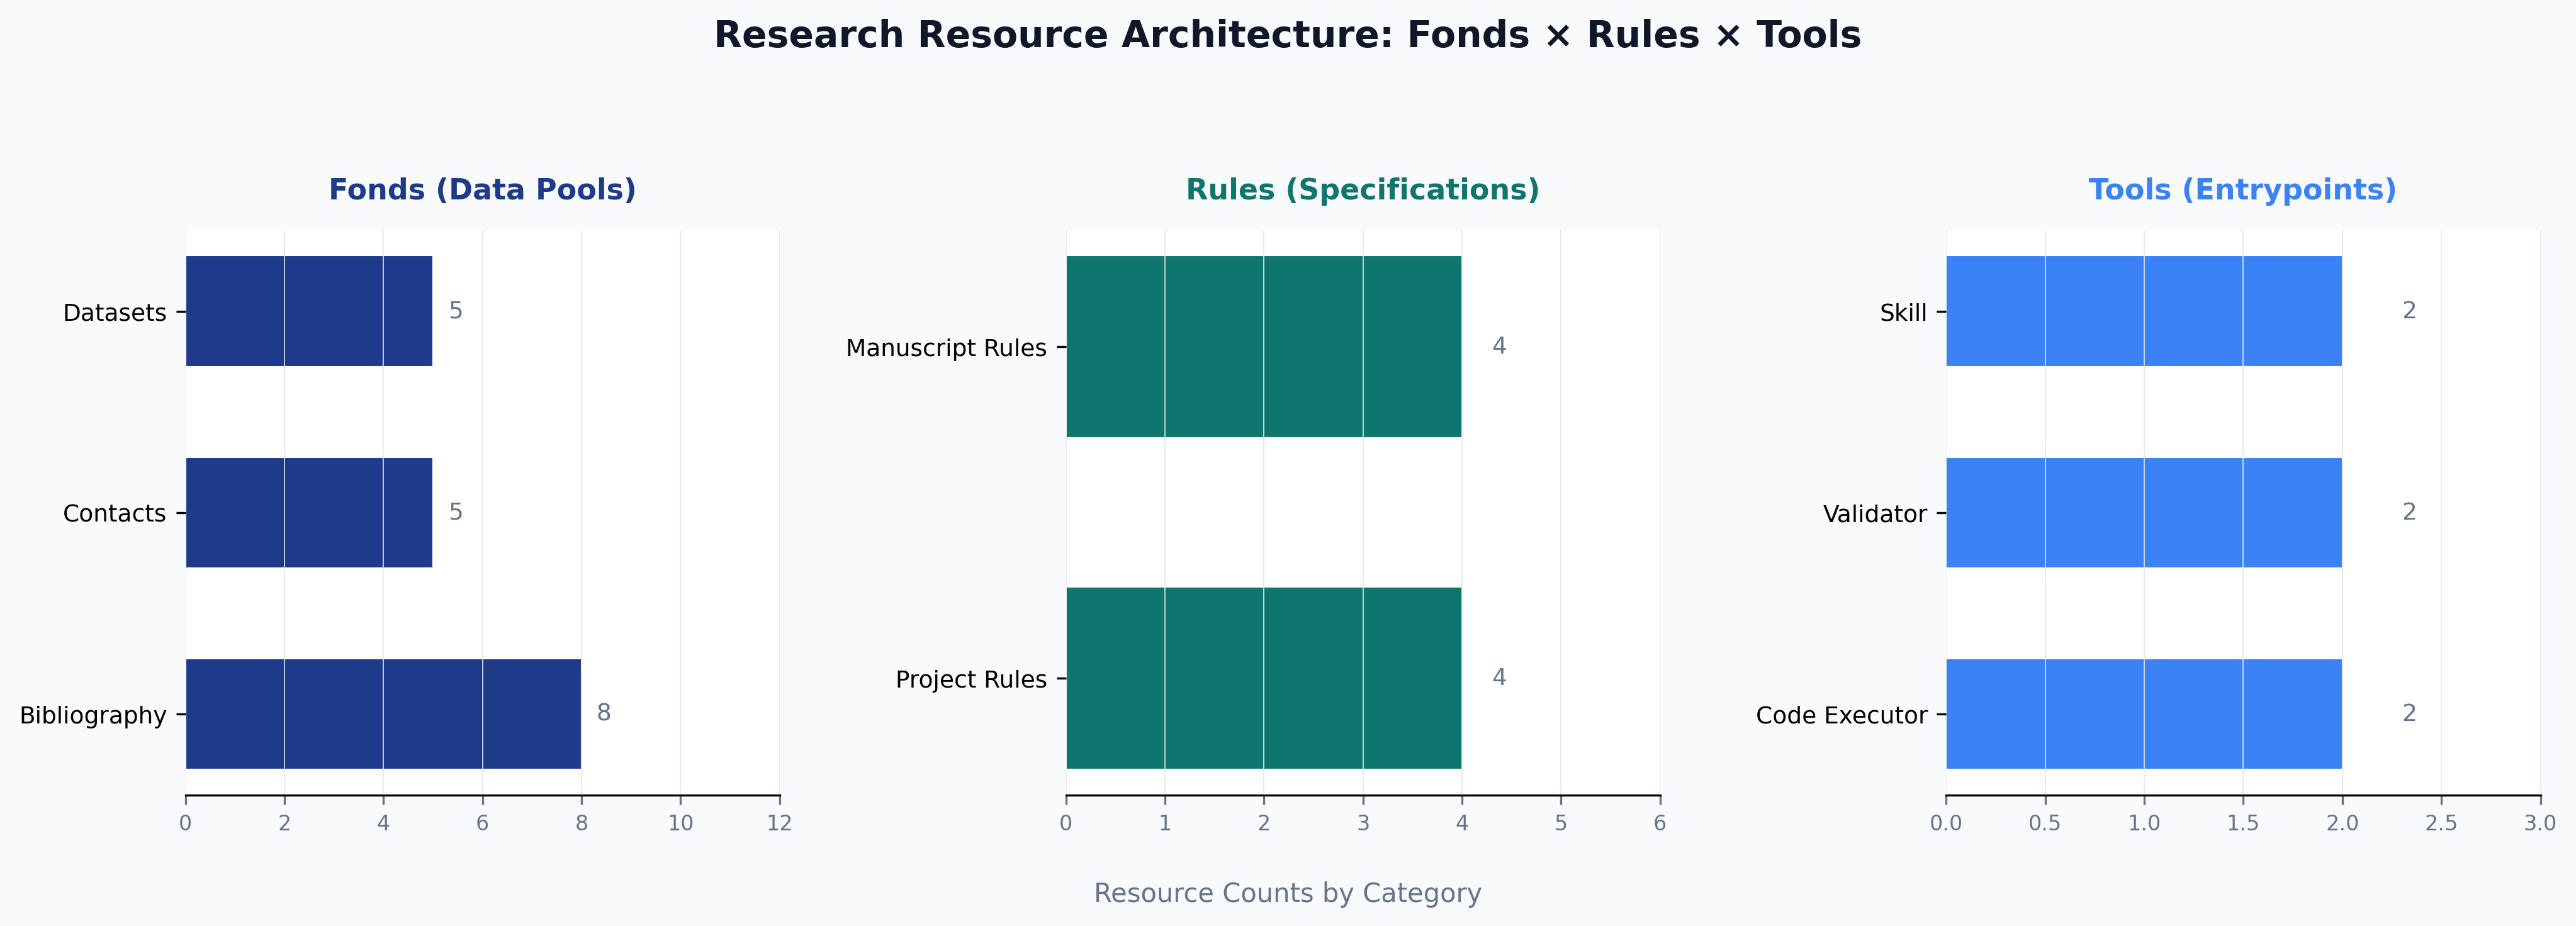
\includegraphics[width=0.9\linewidth,height=0.46\textheight,keepaspectratio,alt={Three-layer resource architecture of template\_pools\_rules\_tools. Fonds (left) provide read-only data pools; Rules (centre) provide governance constraints; Tools (right) provide executable entry points. The Integration layer (bottom) orchestrates all three.}]{../figures/architecture_overview.png}
\caption{Three-layer resource architecture of
template\_pools\_rules\_tools. Fonds (left) provide read-only data
pools; Rules (centre) provide governance constraints; Tools (right)
provide executable entry points. The Integration layer (bottom)
orchestrates all three.}\label{fig:architecture}
\end{figure}

The architecture obeys three design invariants:

\begin{itemize}
\tightlist
\item
  \textbf{Read-only resource access}: no module writes to
  \texttt{fonds/}, \texttt{rules/}, or \texttt{tools/}. The Layer
  Contract in \texttt{AGENTS.md} enforces this at code-review time.
\item
  \textbf{Repo-root-relative discovery}: all path resolution uses
  \texttt{pathlib.Path(\_\_file\_\_).resolve().parents{[}N{]}} so that
  scripts work from any working directory.
\item
  \textbf{Graceful degradation}: every reader checks file existence
  before parsing and catches \texttt{yaml.YAMLError} around the parse
  itself, logging a warning and returning a safe empty value either way.
  The pipeline never raises on a missing or malformed resource.
\end{itemize}
\end{frame}

\begin{frame}[fragile,allowframebreaks]{Related Work and Alternative
Designs}
\protect\phantomsection\label{related-work-and-alternative-designs}
Three broad alternatives to the fonds/rules/tools pattern are common in
research-software monorepos, and each has a known failure mode this
design deliberately avoids.

\textbf{Shared library packages.} A monorepo could publish its
bibliography, contacts, and datasets as an installable Python package
(\breaktt{pip\ install\ monorepo-shared-data}) rather than a filesystem
convention. This works well for stable, versioned data but reintroduces
a packaging and release cycle for data that changes far more often than
code --- every bibliography update would require a version bump and a
re-install across every consuming project, which is precisely the
coordination overhead a monorepo is meant to eliminate.

\textbf{Symlink-based sharing.} Projects could symlink directly into a
shared resource directory rather than discovering it at runtime through
a reader module. This avoids the reader module's implementation cost but
loses the schema-validation and graceful-degradation layers: a symlinked
file that is malformed YAML fails wherever it is read, with no
structured \texttt{status} the pipeline can act on, and no compatibility
check against the manifest's \texttt{version} field.

\textbf{Environment-variable configuration.} Resource locations could be
injected via environment variables (\texttt{FONDS\_ROOT},
\texttt{RULES\_ROOT}) rather than resolved relative to the repository
root. This is the standard twelve-factor-app pattern for services, but
it is a poor fit for a forkable template repository: a contributor who
clones the repository and runs a script expects it to work without any
environment setup, and environment variables are precisely the kind of
implicit, undocumented dependency that a public exemplar should not
require.

The manifest-and-reader pattern adopted here --- versioned typed
manifests, repo-root-relative discovery, and graceful degradation ---
sits between these alternatives: no packaging overhead, structured
validation, and zero required environment configuration.
@fig:pipelineflow shows how this pattern integrates into the project's
script pipeline end-to-end.
\end{frame}

\begin{frame}[fragile,allowframebreaks]{Paper Organisation}
\protect\phantomsection\label{paper-organisation}
The remainder of this paper is structured as follows. @sec:pools
describes the fond layer and the \texttt{fonds\_reader} module,
including the fond schema taxonomy (@fig:taxonomy). @sec:rules describes
the rules layer and the \texttt{rules\_applier} module, including the
soft/strong rule hierarchy (@fig:rulehier). @sec:tools describes the
tool layer and the \texttt{tools\_invoker} module, including the tool
invocation contract (@fig:toolcontract). @sec:integration presents the
unified integration pipeline, the manuscript variable token system, the
three-level resilience design (@fig:resilience), and the script pipeline
(@fig:pipelineflow). @sec:conclusion summarises key findings,
limitations, and future directions.

The architecture overview in @fig:architecture provides a visual map of
these relationships. Runtime statistics collected during integration are
visualised in @fig:counts, and the corresponding per-component
pass/partial/missing states are shown in @fig:pipeline.
\end{frame}

\end{document}
